Fig. \ref{sec3_f2} shows a 5kV MVDC system with a FL based ESM system for controlling operation of the HESS. The detailed modeling of the designed FL based ESM system is discussed in \cite{khan2017fuzzy}. In this section, the design steps of FL based ESM system are discussed briefly.
\begin{figure}[ht!]
\centering
%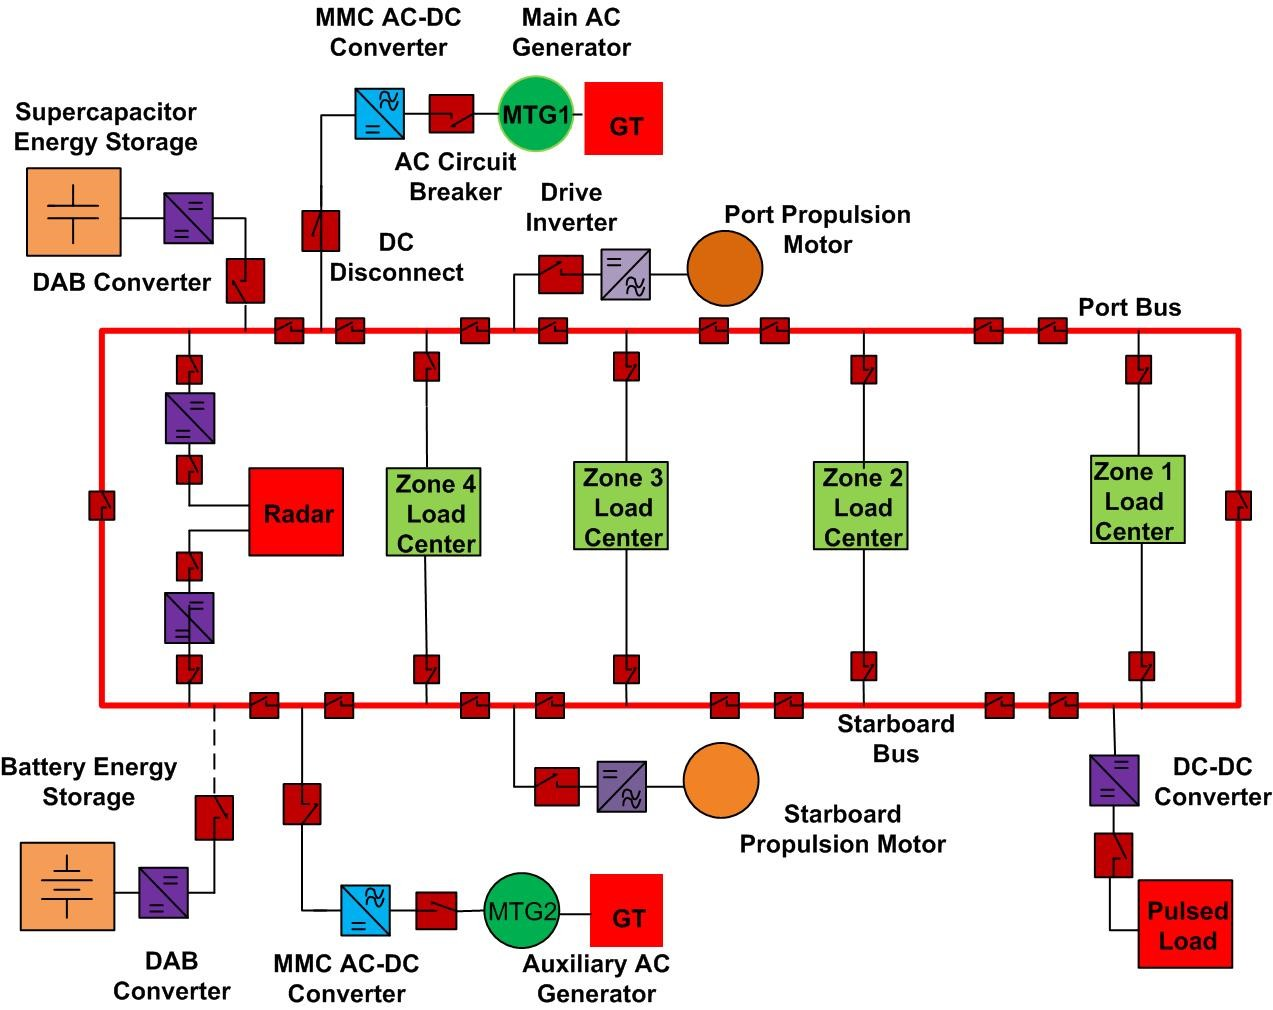
\includegraphics[width=\columnwidth]{f1}
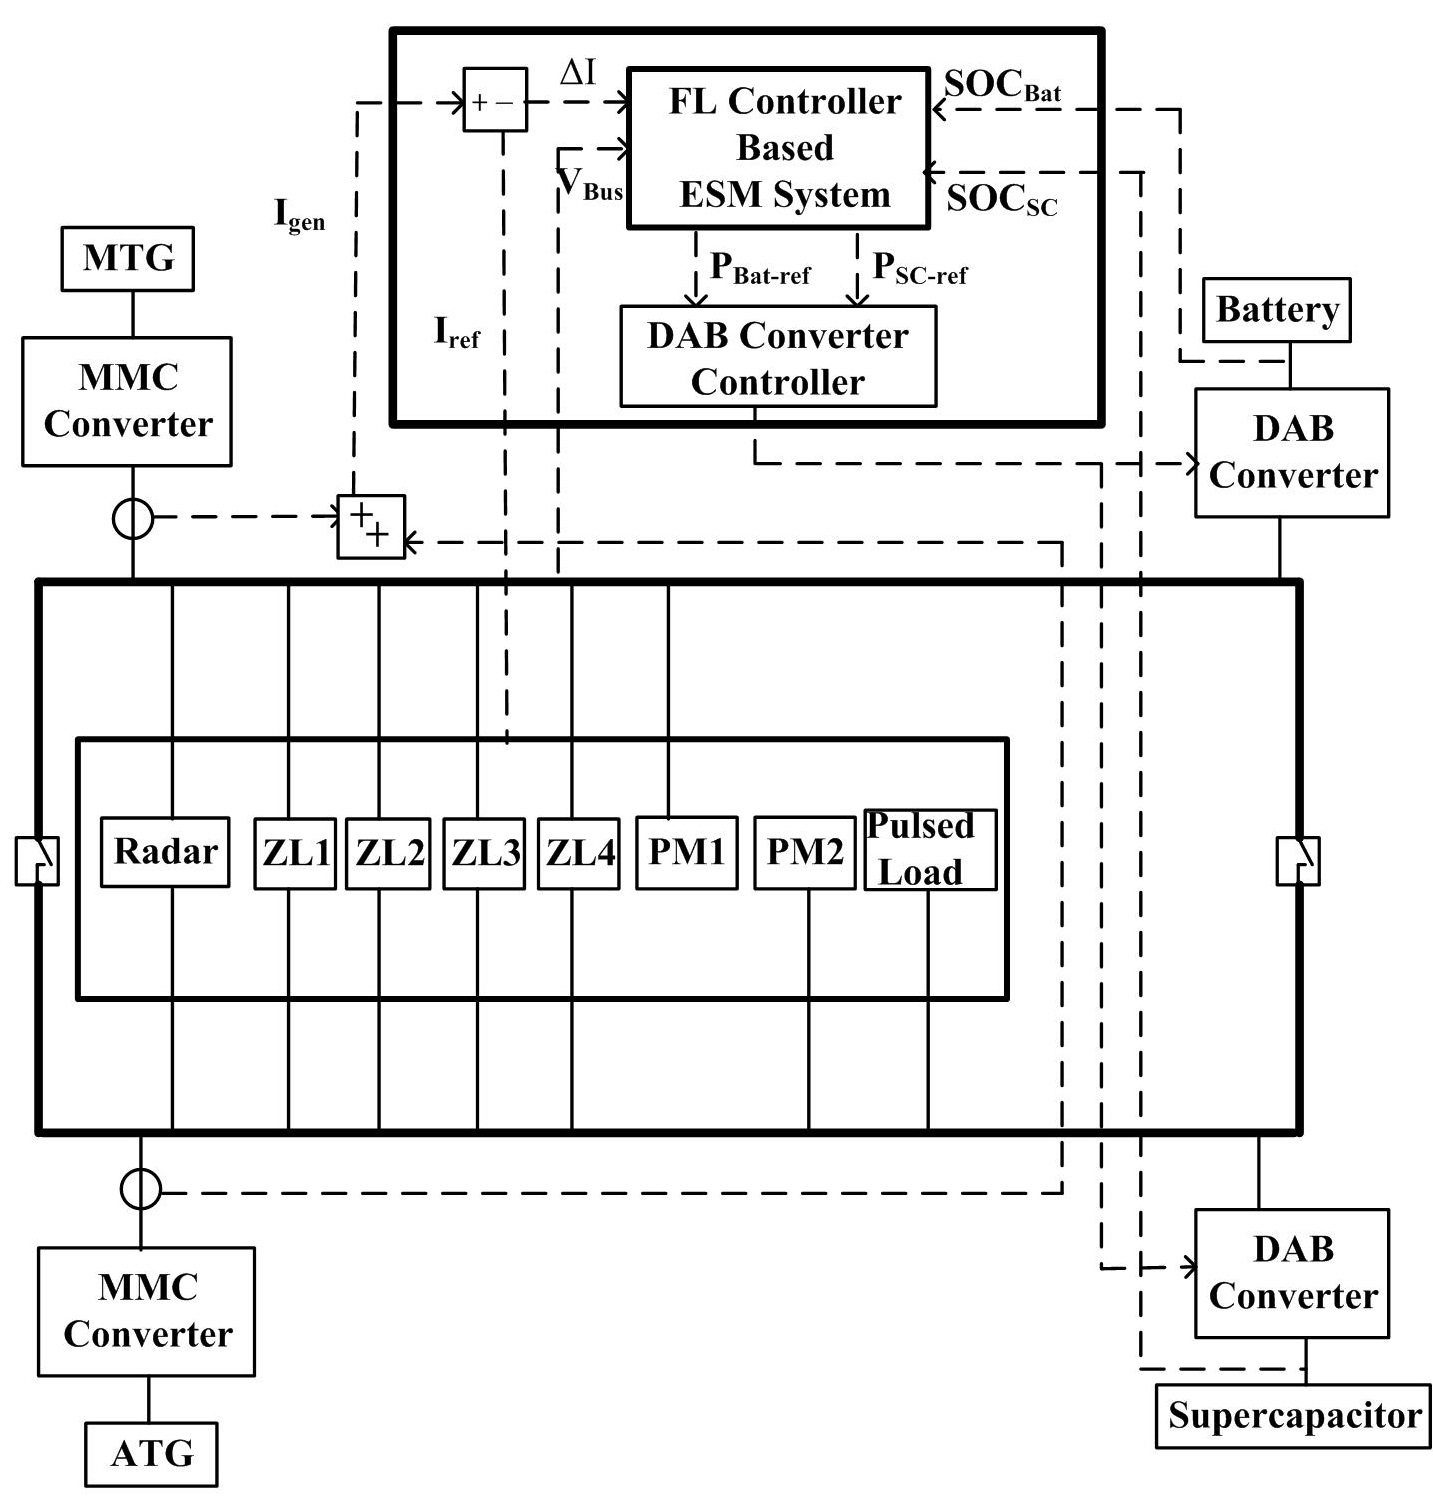
\includegraphics[width=3.51in, height=3.8in]{f2}
\caption{The MVDC system with the FL controller based ESM system.}
\label{sec3_f2}
\end{figure} 

Fig. \ref{sec3_f3} shows the block diagram of the ESM system which has two main steps. In the first step, the total storage reference power ($P_{stor-ref}$) is determined by using the FL controller. Where, $P_{stor-ref}$ represents total charging or discharging power of the battery and supercapacitor combined. After the first step, there is a generation limit checking controller to ensure that the sum of the power demand of the loads and charging reference power of the HESS is within the generation limit (40MW). After passing the $P_{stor-ref}$ through the generation limit checking controller, the aim is to divide $P_{stor-ref}$ between the assigned energy storages as the battery reference power ($P_{Bat-ref}$) and the supercapacitor reference power ($P_{SC-ref}$). To do this, the $P_{stor-ref}$ is passed through a low pass filter (LPF) which separates the respective power for each of them.
\begin{figure}[ht!]
\centering
%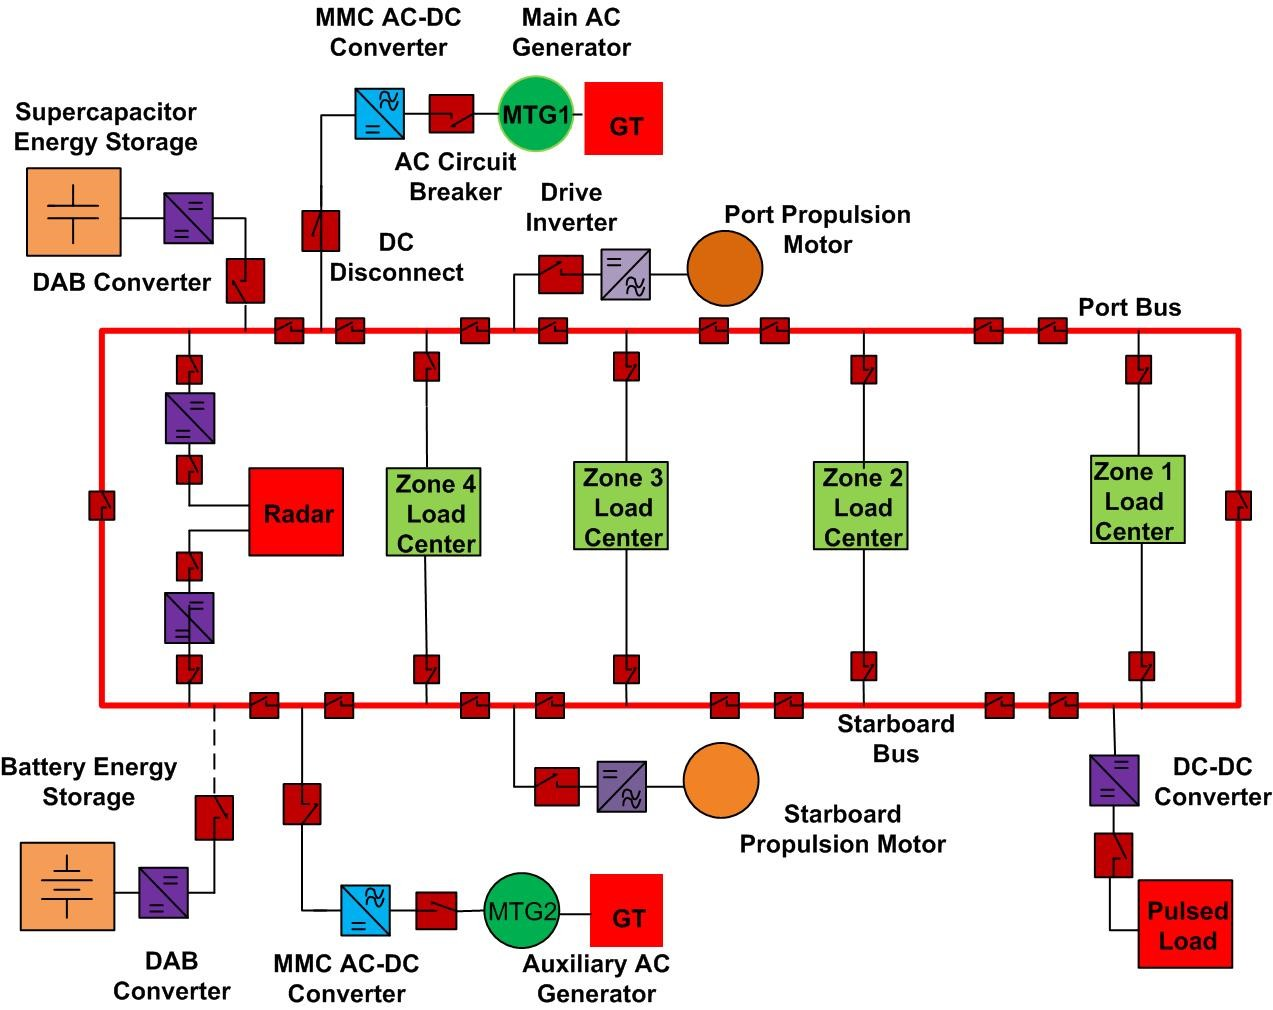
\includegraphics[width=\columnwidth]{f1}
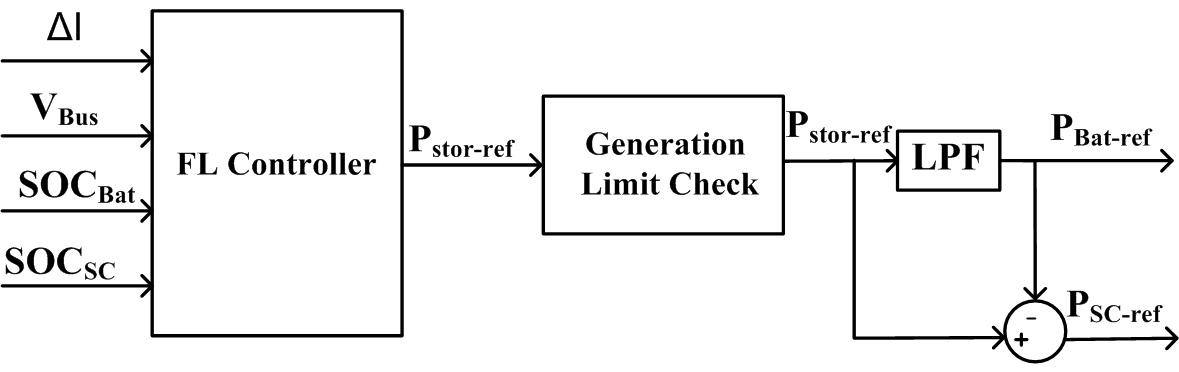
\includegraphics[width=3.46in, height=1.19in]{f3}
\caption{FL controller and LPF based ESM system.}
\label{sec3_f3}
\end{figure}
\subsection{Estimation of $P_{stor-ref}$}
The intention of using FL controller in the first step is to generate the total charging or discharging power of the energy storages based on the condition of the mismatch of the measured load power and actual demanded power and the mismatch of the reference bus voltage of the MVDC system (5kV) and the measured bus voltage. It is also needed to keep the SOC of the energy storages within the limit to avoid the danger of deep discharging and overcharging. Considering these objectives, four input variables based FL controller is designed. The input variables are: $\Delta I$, $V_{Bus}$, $SOC_{Bat}$, and $SOC_{SC}$. Where, $\Delta I$ means the difference between the total reference current ($I_{ref}$) and  the total generated current ($I_{gen}$), $V_{Bus}$ means measured MVDC bus voltage, $SOC_{SC}$ and $SOC_{Bat}$ mean the measured SOC of the supercapacitor and the battery respectively. The output variable is $P_{stor-ref}$ which is the total reference power of the energy storages. The three steps of FL based control technique are discussed here. 

\subsubsection{Fuzzyfication}
\begin{figure}[ht!]
\centering
%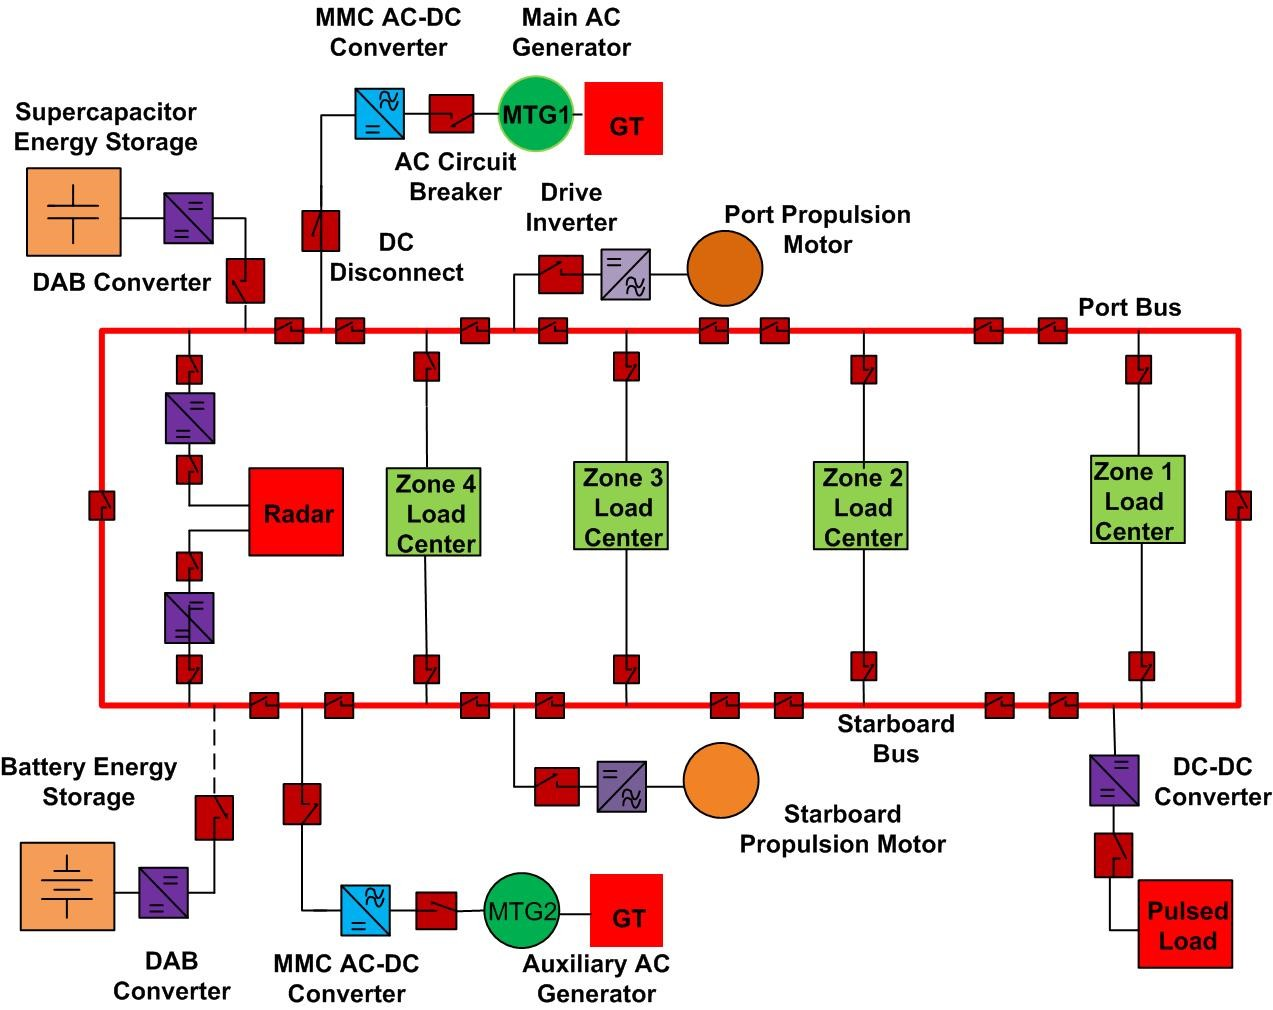
\includegraphics[width=\columnwidth]{f1}
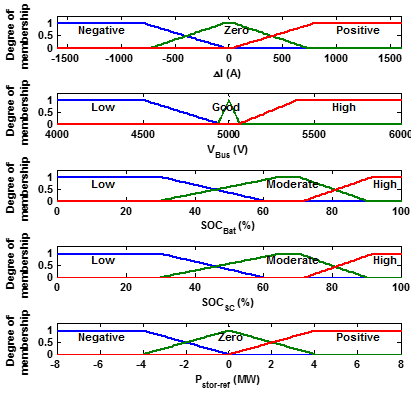
\includegraphics[width=3.46in, height=3.64in]{f4}
\caption{Input and output variables membership functions for the FL controller.}
\label{sec3_f4}
\end{figure}
Fig. \ref{sec3_f4} shows the input and output variables membership functions of the designed FL controller. The operating range of the first input variables, $\Delta I$ is divided into three membership functions, Positive, Negative and Zero. All the membership functions are trapezoidal shaped. The upper and lower limit of the input variable, $\Delta I$ are 1600A and -1600A, respectively. The limits are determined based on the maximum mismatch of the total measured power and total demanded power, the capacity of the energy storages. The second input variable, $V_{Bus}$ also has three membership functions, Low, Good, and High where the Low and High membership functions are the trapezoidal shape and Good membership function is a triangular shape. The upper limit and lower limit of $V_{Bus}$ are  6kV and 4kV, respectively. The third and fourth input variables ($SOC_{Bat}$ and $SOC_{SC}$) have three membership functions where all the membership functions are the trapezoidal shape. The upper limit and lower limit of the third and fourth input variables are 100\% and 0\%, respectively. The output variable, $P_{stor-ref}$ has three membership functions, Positive, Negative and Zero where the Positive and Negative membership functions are the trapezoidal shape and the Zero membership function is a triangular shape.
\subsubsection{Inference} 
The designed FL controller has four input variables and one output variable and each variable has 3 membership functions. Total 81 fuzzy rules are designed to estimate the output variable, $P_{stor-ref}$. As the designed FL controller is associated with five variables and a 2-D table is not sufficient to explain all the fuzzy rules, the fuzzy rules are shown in Table \ref{fl1 controller table}. In the Table \ref{fl1 controller table}, the meaning of the symbols are  N = Negative, Z = Zero, P = Positive, L = Low, G = Good, H = High, and M = Moderate. For example, the first fuzzy rule is: 
\begin{itemize}
\item {\textbf{IF}} $\Delta I$ is N (Negative) {\textbf{AND}} $V_{Bus}$ is L (Low) {\textbf{AND}}  $SOC_{Bat}$ is L (Low) {\textbf{AND}} $SOC_{SC}$ is L (Low), {\textbf{THEN}} $P_{stor-ref}$ is Z (Zero)
\end{itemize}
%table 
\begin{table}[ht!]
%\centering
\processtable{Fuzzy Rules: $P_{stor-ref}$\label{fl1 controller table}}
{\begin{tabu}{p{4.1cm}|p{0.45cm}|p{0.45cm}|[2pt]p{0.45cm}|p{0.45cm}|p{0.45cm}}
\hline
{} &\multicolumn{2}{c|}{\multirow{2}{*}{$\bf P_{stor-ref}$}} & \multicolumn{3}{c}{$\Delta I$} \\
\cmidrule{4-6} 
{}&\multicolumn{2}{c|}{} & N& Z& P\\
\cmidrule{2-6}
\cmidrule{4-6}\tabucline[2pt]{4-6}
{When}&\multirow{3}{*}{$V_{Bus}$} & L& \bf Z & \bf Z & \bf P\\ 
\cmidrule{3-6}
{$SOC_{Bat}$=L AND $SOC_{SC}$=L}&{}& G & \bf Z& \bf Z & \bf P \\ 
\cmidrule{3-6}
&{}& H & \bf Z& \bf Z & \bf P \\
\hline\tabucline[2pt]{4-6}
{When} &\multicolumn{2}{c|}{\multirow{2}{*}{$\bf P_{stor-ref}$}} & \multicolumn{3}{c}{$\Delta I$} \\
\cmidrule{4-6} 
{$SOC_{Bat}$ =L AND $SOC_{SC}$=M/H,}&\multicolumn{2}{c|}{} & N& Z& P\\
\cmidrule{2-6}\tabucline[2pt]{4-6}
{$SOC_{Bat}$=M/H AND $SOC_{SC}$=L,}&\multirow{3}{*}{$V_{Bus}$} & L& \bf N & \bf N & \bf P\\ 
\cmidrule{3-6}
{$SOC_{Bat}$=M AND $SOC_{SC}$=M}&{}& G & \bf N& \bf Z & \bf P \\ 
\cmidrule{3-6}
{}&{}& H & \bf N& \bf Z & \bf P \\
\hline\tabucline[2pt]{4-6}
{ } &\multicolumn{2}{c|}{\multirow{2}{*}{$\bf P_{stor-ref}$}} & \multicolumn{3}{c}{$\Delta I$} \\
\cmidrule{4-6} 
{When}&\multicolumn{2}{c|}{} & N& Z& P\\
\cmidrule{2-6}\tabucline[2pt]{4-6}
{$SOC_{Bat}$=H AND $SOC_{SC}$=M,}&\multirow{3}{*}{$V_{Bus}$} & L& \bf N & \bf N & \bf Z\\ 
\cmidrule{3-6}
{$SOC_{Bat}$=M AND $SOC_{SC}$=H}&{}& G & \bf N& \bf Z & \bf P \\ 
\cmidrule{3-6}
{}&{}& H & \bf N& \bf Z & \bf P \\
\hline\tabucline[2pt]{4-6}
{} &\multicolumn{2}{c|}{\multirow{2}{*}{$\bf P_{stor-ref}$}} & \multicolumn{3}{c}{$\Delta I$} \\
\cmidrule{4-6} 
{}&\multicolumn{2}{c|}{} & N& Z& P\\
\cmidrule{2-6} \tabucline[2pt]{4-6}
{When}&\multirow{3}{*}{$V_{Bus}$} & L& \bf N & \bf N & \bf Z\\ 
\cmidrule{3-6}
{$SOC_{Bat}$=H AND $SOC_{SC}$=H}&{}& G & \bf N& \bf Z & \bf Z \\ 
\cmidrule{3-6}
&{}& H & \bf N& \bf Z & \bf Z \\
\hline\tabucline[2pt]{4-6}

\end{tabu}}{}
\end{table}
\subsubsection{Defuzzyfication}
Fig. \ref{sec3_f4} and Fig. \ref{sec3_f5} show the membership functions of the output variable, $P_{stor-ref}$ and the surface plot for the FL controller, respectively.  Fig. \ref{sec3_f5} shows the response of $P_{stor-ref}$ versus $\Delta I$ and $V_{Bus}$ when $SOC_{Bat}$ and $SOC_{SC}$ are set to 75\% and 82.65\%, respectively.
\begin{figure}[ht!]
\centering
%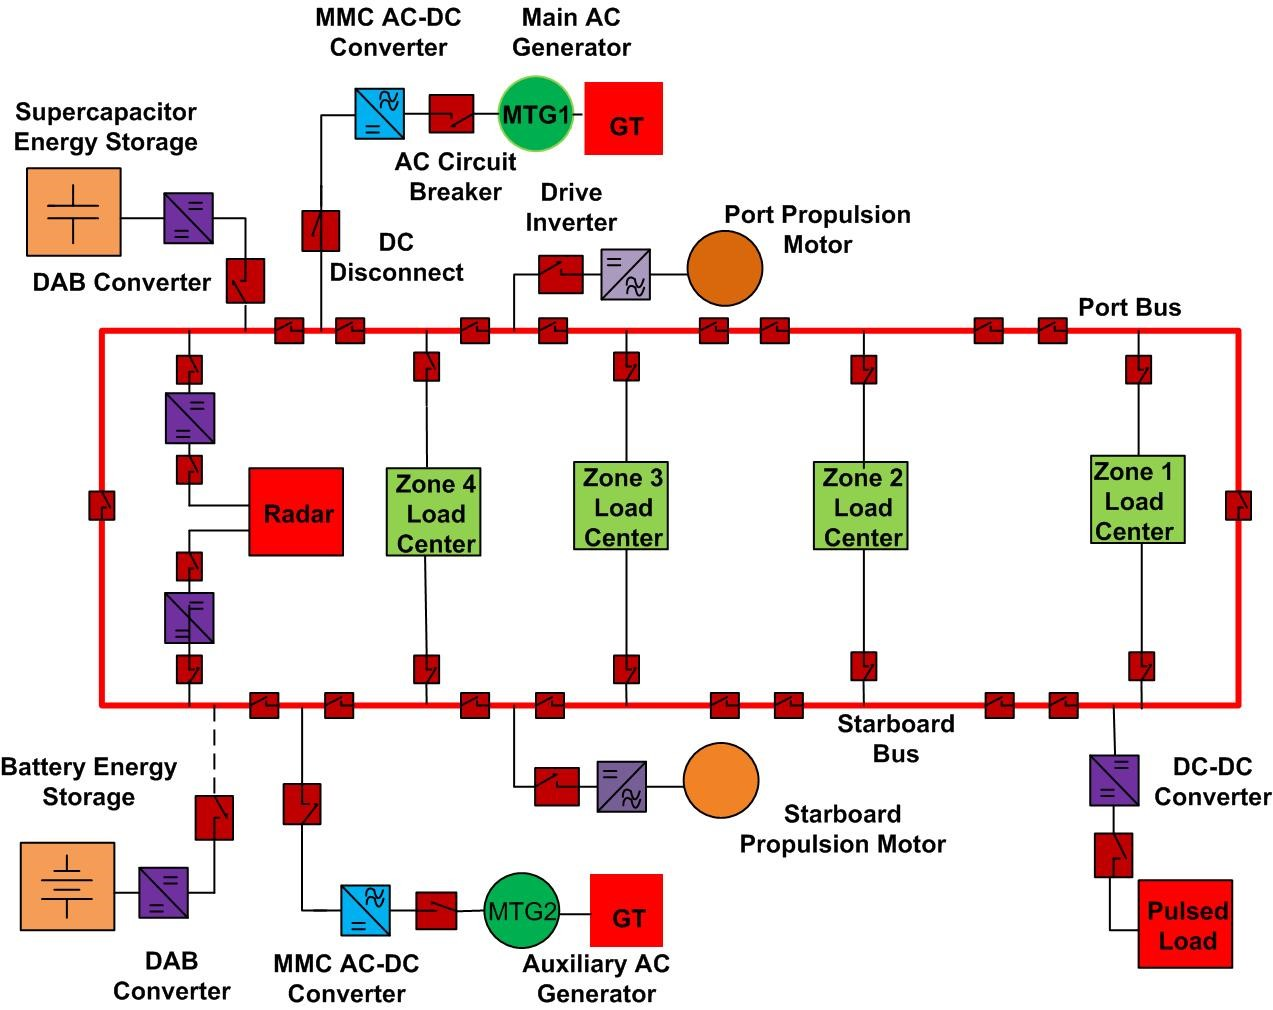
\includegraphics[width=\columnwidth]{f1}
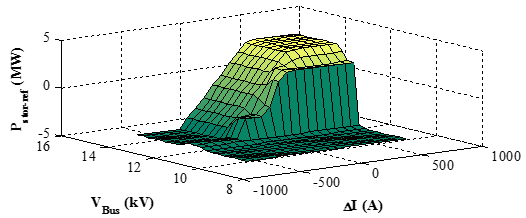
\includegraphics[width=3.46in, height=1.5in]{f5}
\caption{Generated surface of FL controller for $P_{stor-ref}$ versus $\Delta I$, and $V_{Bus}$ when $SOC_{Bat}$, and $SOC_{SC}$ are set to 75\% and 82.65\%, respectively.} 
\label{sec3_f5}
\end{figure} 
\subsection{Estimation of $P_{Bat-ref}$ and $P_{SC-ref}$}
In the second step the $P_{stor-ref}$ is passed through a LPF. The output of the LPF is a low frequency component of $P_{stor-ref}$ which is assigned as the battery reference power, $P_{Bat-ref}$. The difference of $P_{stor-ref}$ and $P_{Bat-ref}$ is the high frequency component of $P_{stor-ref}$ which is assigned as  $P_{SC-ref}$. The transfer function of the LPF is given in (\ref{equation-1}), where $f_{cf}$ is the LPF’s cutoff frequency. As the average models of the converters' are used, the value of cutoff frequency ($f_{cf}$) is set as 1Hz.  
\begin{equation} \label{equation-1}
G_f=\frac {2\pi f_{cf}}{s+2\pi f_{cf}}
\end{equation}
